\section{Related Work}
\label{2017-batched-spmv:sec:related}


\begin{figure}[t]
\centering
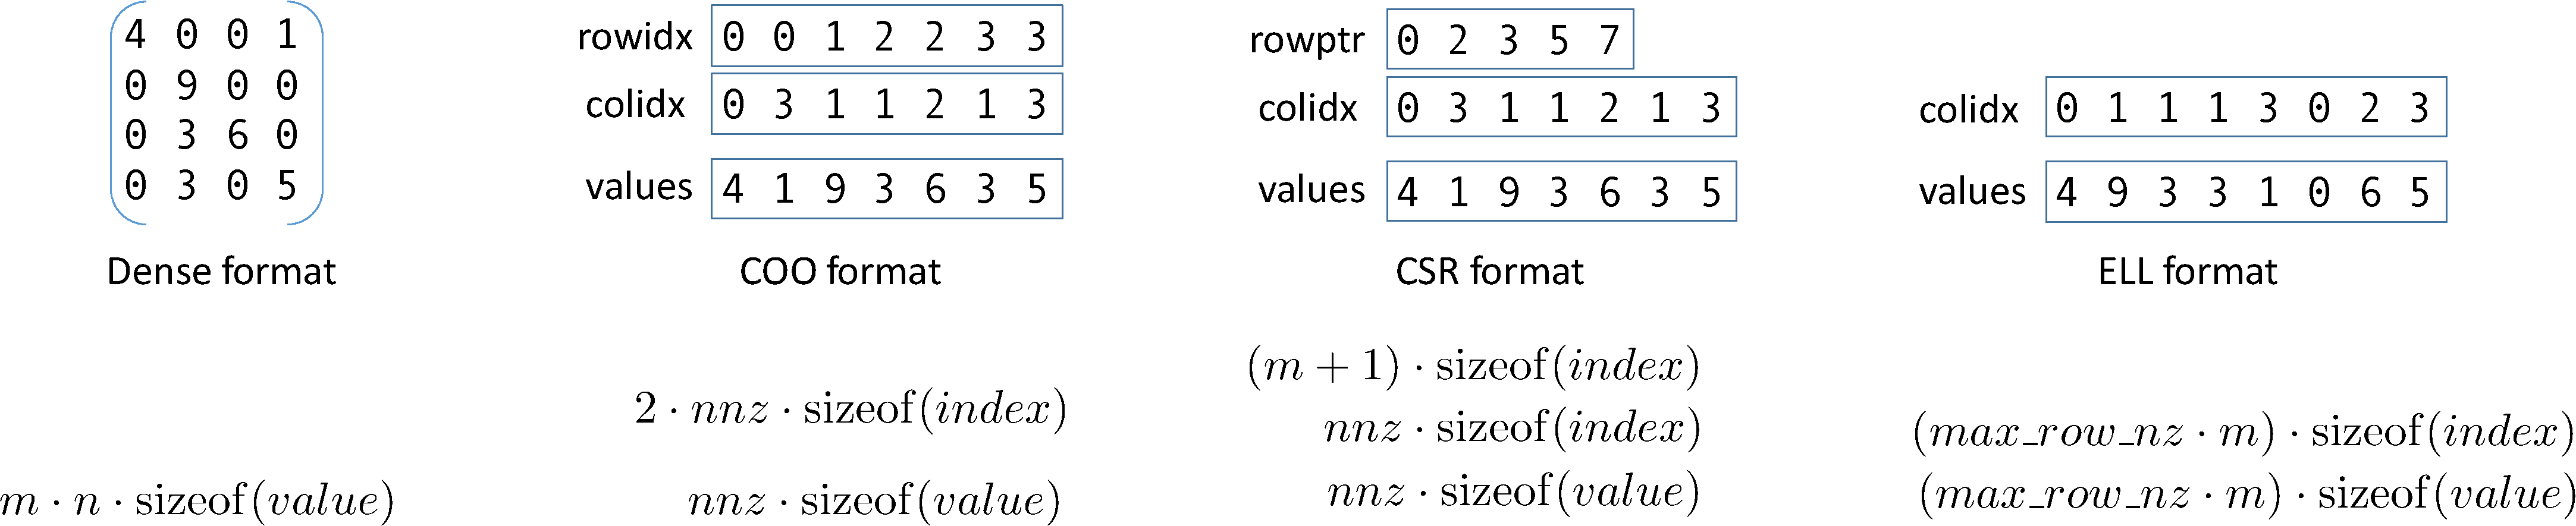
\includegraphics[width=\columnwidth]{plots/formats}
\caption
[Basic storage formats and memory consumption for sparse matrices]
{Basic storage formats for an $m\times n$ sparse matrix with $nnz$
    nonzeros along with memory consumption.}
\label{2017-batched-spmv:fig:formatoverview}
\end{figure}

\subsection{\spmv on manycore architectures}

Improving the performance of \spmv on modern architectures is an active field of research. 
A critical factor is the selection of an appropriate
sparse matrix format, which reduces the storage cost by maintaining only the nonzero values
but has to keep some additional information in order to derive the location of the elements.

The simplest idea is to explicitly store only the nonzero elements
along with the row and column indices (i.e. coordianates) of each element.
This coordinate (COO)
format~\cite{barrettemplates} allows to determine the original position of any element
in the matrix without processing any other entries.

If the elements are sorted row-wise and, for performance reasons,
in increasing column-order within each row,
the storage cost can be reduced.
The ``Compressed Sparse Row'' (CSR~\cite{barrettemplates})
format
replaces the array containing the row indices with a pointer to the beginning 
of the distinct rows, reducing the amount of data required to store the row
information, at the cost of
additional processing necessary to determine the row location of the elements.

While being very
popular for manycore architectures in general, the ELL format~\cite{ellpack}
is particularly suited for GPUs.
In this layout, the distinct rows are padded with zeros to ensure
they are all of the same length.
While this typically increases the storage cost, 
it removes the need to maintain the row pointers,
and enables processing the column-indices (and values) in distinct
rows in SIMD fashion. Furthermore,
coalescent memory access is attained if the matrix containing
the nonzero elements
is stored in column-major order.

The three basic formats targeted in our batched kernels are illustrated
in Figure~\ref{2017-batched-spmv:fig:formatoverview}. In addition to these basic formats, there exist many other variants,
which often arise as a combination of the basic formats.
For example, the hybrid format stores the matrix partly in ELL and partly in CSR/COO; 
and the sliced ELL format (SELL-p) ~\cite{sellcs} chops the matrix into row blocks and stores each block in ELL
format.


Related to the storage format is the question of how to parallelize
\spmv.
The main challenges in this context are: 
1) balancing the workload among the distinct cores/threads; and 
2) ensuring an efficient access to the matrix entries and the vector values.
The second aspect is in particular relevant on NVIDIA GPUs where each memory access
reads 128 contiguous bytes of memory~\cite{cuda8.0}.
In case of fine-grained parallelism, balancing the workload naturally results in 
multiple threads computing partial sums for one row, which requires careful synchronization
when writing the result entry back into main memory.
In this paper, we exclusively focus on (batched) \spmv implementations for 
GPU architectures. For a comprehensive overview about
the CUDA programming model and its implications, see~\cite{cuda8.0,lawn2016}.

\label{2017-batched-spmv:sec:s2-related}
\subsection{Batched routines}

The development of specialized routines for an operation involving many
problems
of small size that are pairwise independent, and can thus be handled simultaneously, 
has recently gained a lot of attention
due to their heavy application in machine learning~\cite{Abdelfattah2016}.
The motivation for designing these kernels is that the amount of hardware concurrency
in manycore processors such as GPUs
often exceeds the level of parallelism exploited by conventional routines.
Consequently, handling the distinct problems in sequence
utilizes only a fraction of the hardware resources and incurs a significant kernel launch overhead.
In response to this, there are several
efforts among the high performance computing community to
standardize the interface for a batched version of the basic linear algebra subprograms (BLAS)
and more complex functionality built on top of it~\cite{bblas}.
